\documentclass[10pt,utf8,notheorems,compress,t]{beamer}
\usepackage{etex}

\usepackage{pgfpages}
%\setbeameroption{show notes on second screen}
\setbeamertemplate{note page}[plain]
\newcommand{\jnote}[2]{\only<#1>{\note{\setlength\parskip{\medskipamount}\justifying\footnotesize#2\par}}}
%\newcommand{\jnote}[2]{}

% Workaround for the issue described at
% https://tex.stackexchange.com/questions/164406/beamer-using-href-in-notes.
\newcommand{\fixedhref}[2]{\makebox[0pt][l]{\hspace*{\paperwidth}\href{#1}{#2}}\href{#1}{#2}}

\usepackage[english]{babel}

\usepackage{graphbox}
\usepackage{mathtools}
\usepackage{booktabs}
\usepackage{stmaryrd}
\usepackage{array}
\usepackage{ragged2e}
\usepackage{multicol}
\usepackage{tabto}
\usepackage{xstring}
\usepackage{ifthen}
\usepackage[normalem]{ulem}
\usepackage[all]{xy}
\xyoption{rotate}
\usepackage{tikz}
\usetikzlibrary{calc,shapes,shapes.callouts,shapes.arrows,patterns,fit,backgrounds,decorations.pathmorphing,positioning}
\hypersetup{colorlinks=true}

\usepackage{pifont}
\newcommand{\cmark}{\ding{51}}
\newcommand{\xmark}{\ding{55}}
\DeclareSymbolFont{extraup}{U}{zavm}{m}{n}
\DeclareMathSymbol{\varheart}{\mathalpha}{extraup}{86}

\graphicspath{{images/}}

\usepackage[protrusion=true,expansion=true]{microtype}

\setlength\parskip{\medskipamount}
\setlength\parindent{0pt}

\title{Without loss of generality, any reduced ring is a field}
\author{Ingo Blechschmidt}
\date{February 2nd, 2022}

\useinnertheme{rectangles}
\setbeamerfont{block title}{size={}}

\useinnertheme{rectangles}

\usecolortheme{orchid}
\usecolortheme{seahorse}
\definecolor{mypurple}{RGB}{150,0,255}
\setbeamercolor{structure}{fg=mypurple}
\definecolor{myred}{RGB}{150,0,0}
\setbeamercolor*{title}{bg=mypurple,fg=white}
\setbeamercolor*{titlelike}{bg=mypurple,fg=white}
\setbeamercolor{frame}{bg=black}

\usefonttheme{serif}
\usepackage[T1]{fontenc}
\usepackage{libertine}

% lifted from https://arxiv.org/abs/1506.08870
\DeclareFontFamily{U}{min}{}
\DeclareFontShape{U}{min}{m}{n}{<-> udmj30}{}
\newcommand\yon{\!\text{\usefont{U}{min}{m}{n}\symbol{'210}}\!}

\newcommand{\A}{\mathcal{A}}
\newcommand{\B}{\mathcal{B}}
\newcommand{\C}{\mathcal{C}}
\newcommand{\M}{\mathcal{M}}
\renewcommand{\AA}{\mathbb{A}}
\newcommand{\E}{\mathcal{E}}
\newcommand{\F}{\mathcal{F}}
\newcommand{\G}{\mathcal{G}}
\newcommand{\J}{\mathcal{J}}
\newcommand{\GG}{\mathbb{G}}
\renewcommand{\O}{\mathcal{O}}
\newcommand{\K}{\mathcal{K}}
\newcommand{\NN}{\mathbb{N}}
\newcommand{\QQ}{\mathbb{Q}}
\newcommand{\RR}{\mathbb{R}}
\newcommand{\TT}{\mathbb{T}}
\newcommand{\PP}{\mathbb{P}}
\newcommand{\ZZ}{\mathbb{Z}}
\newcommand{\CC}{\mathbb{C}}
\renewcommand{\P}{\mathcal{P}}
\newcommand{\aaa}{\mathfrak{a}}
\newcommand{\ppp}{\mathfrak{p}}
\newcommand{\fff}{\mathfrak{f}}
\newcommand{\defeq}{\vcentcolon=}
\newcommand{\defeqv}{\vcentcolon\equiv}
\newcommand{\Sh}{\mathrm{Sh}}
\newcommand{\GL}{\mathrm{GL}}
\newcommand{\Zar}{\mathrm{Zar}}
\newcommand{\op}{\mathrm{op}}
\newcommand{\Set}{\mathrm{Set}}
\newcommand{\Eff}{\mathrm{Ef{}f}}
\newcommand{\Sch}{\mathrm{Sch}}
\newcommand{\Aff}{\mathrm{Aff}}
\newcommand{\Ring}{\mathrm{Ring}}
\newcommand{\LocRing}{\mathrm{LocRing}}
\newcommand{\LRS}{\mathrm{LRS}}
\newcommand{\Hom}{\mathrm{Hom}}
\newcommand{\Spec}{\mathrm{Spec}}
\newcommand{\lra}{\longrightarrow}
\newcommand{\RelSpec}{\operatorname{Spec}}
\renewcommand{\_}{\mathpunct{.}}
\newcommand{\?}{\,{:}\,}
\newcommand{\ul}[1]{\underline{#1}}
\newcommand{\affl}{\ensuremath{{\ul{\ensuremath{\AA}}^1}}}
\newcommand{\Ll}{\text{iff}}
\newcommand{\inv}{inv.\@}
\newcommand{\seq}[1]{\mathrel{\vdash\!\!\!_{#1}}}
\newcommand{\hg}{\mathbin{:}}  % homogeneous coordinates
\newcommand{\brak}[1]{{\llbracket{#1}\rrbracket}}
\newcommand{\pt}{\mathrm{pt}}
\newcommand{\Loc}{\mathrm{Loc}}
\newcommand{\Top}{\mathrm{Top}}

%\setbeamertemplate{blocks}[rectangles][shadow=false]

\newenvironment{indentblock}{%
  \list{}{\leftmargin\leftmargin}%
  \item\relax
}{%
  \endlist
}

% Adapted from https://latex.org/forum/viewtopic.php?t=2251 (Stefan Kottwitz)
\newenvironment<>{hilblock}{
  \begin{center}
    \begin{minipage}{9.05cm}
      \setlength{\textwidth}{9.05cm}
      \begin{actionenv}#1
        \def\insertblocktitle{}
        \par
        \usebeamertemplate{block begin}}{
        \par
        \usebeamertemplate{block end}
      \end{actionenv}
    \end{minipage}
  \end{center}}

\newcommand{\bignumber}[1]{
  \renewcommand{\insertenumlabel}{#1}\scalebox{1.5}{\usebeamertemplate{enumerate item}}
}
\newcommand{\bigheart}{
\includegraphics{heart}}

\newenvironment{changemargin}[2]{%
  \begin{list}{}{%
    \setlength{\topsep}{0pt}%
    \setlength{\leftmargin}{#1}%
    \setlength{\rightmargin}{#2}%
    \setlength{\listparindent}{\parindent}%
    \setlength{\itemindent}{\parindent}%
    \setlength{\parsep}{\parskip}%
  }%
  \item[]}{\end{list}}

\tikzset{
  invisible/.style={opacity=0,text opacity=0},
  visible on/.style={alt={#1{}{invisible}}},
  alt/.code args={<#1>#2#3}{%
    \alt<#1>{\pgfkeysalso{#2}}{\pgfkeysalso{#3}}}
}

\newcommand{\pointthis}[3]{%
  \tikz[remember picture,baseline]{
    \node[anchor=base,inner sep=0,outer sep=0] (#2) {#2};
    \node[visible on=#1,overlay,rectangle callout,rounded corners,callout relative pointer={(0.3cm,0.5cm)},fill=blue!20] at ($(#2.north)+(-0.1cm,-1.1cm)$) {#3};
  }%
}

\tikzset{
  invisible/.style={opacity=0,text opacity=0},
  visible on/.style={alt={#1{}{invisible}}},
  alt/.code args={<#1>#2#3}{%
    \alt<#1>{\pgfkeysalso{#2}}{\pgfkeysalso{#3}}}
}

\newcommand{\hcancel}[5]{%
  \tikz[baseline=(tocancel.base)]{
    \node[inner sep=0pt,outer sep=0pt] (tocancel) {#1};
    \draw[red!80, line width=0.4mm] ($(tocancel.south west)+(#2,#3)$) -- ($(tocancel.north east)+(#4,#5)$);
  }%
}

\newcommand{\explain}[7]{%
  \tikz[remember picture,baseline]{
    \node[anchor=base,inner sep=2pt,outer sep=0,fill=#3,rounded corners] (label) {#1};
    \node[anchor=north,visible on=<#2>,overlay,rectangle callout,rounded corners,callout
    relative pointer={(0.0cm,0.5cm)+(0.0cm,#6)},fill=#3] at ($(label.south)+(0,-0.3cm)+(#4,#5)$) {#7};
  }%
}

\newcommand{\explainstub}[2]{%
  \tikz[remember picture,baseline]{
    \node[anchor=base,inner sep=2pt,outer sep=0,fill=#2,rounded corners] (label) {#1};
  }%
}

\newcommand{\squiggly}[1]{%
  \tikz[remember picture,baseline]{
    \node[anchor=base,inner sep=0,outer sep=0] (label) {#1};
    \draw[thick,color=red!80,decoration={snake,amplitude=0.5pt,segment
    length=3pt},decorate] ($(label.south west) + (0,-2pt)$) -- ($(label.south east) + (0,-2pt)$);
  }%
}

\setbeamertemplate{frametitle}[default][center]

% Adapted from https://latex.org/forum/viewtopic.php?t=2251 (Stefan Kottwitz)
\newenvironment<>{varblock}[2]{\begin{varblockextra}{#1}{#2}{}}{\end{varblockextra}}
\newenvironment<>{varblockextra}[3]{
  \begin{center}
    \begin{minipage}{#1}
      \begin{actionenv}#4
	\def\insertblocktitle{\vspace*{-1em}}
        \def\varblockextraend{#3}
	\usebeamertemplate{block begin}}{
        \par
        \usebeamertemplate{block end}
        \varblockextraend
      \end{actionenv}
    \end{minipage}
  \end{center}}


\setbeamertemplate{navigation symbols}{}

\newcounter{framenumberpreappendix}
\newcommand{\backupstart}{
  \setcounter{framenumberpreappendix}{\value{framenumber}}
}
\newcommand{\backupend}{
  \addtocounter{framenumberpreappendix}{-\value{framenumber}}
  \addtocounter{framenumber}{\value{framenumberpreappendix}}
}

\newcommand{\insertframeextra}{}
\setbeamertemplate{footline}{%
  \begin{beamercolorbox}[wd=\paperwidth,ht=2.25ex,dp=1ex,right,rightskip=1mm,leftskip=1mm]{}%
    % \inserttitle
    \hfill
    \insertframenumber\insertframeextra\,/\,\inserttotalframenumber
  \end{beamercolorbox}%
  \vskip0pt%
}


\newcommand{\hil}[1]{{\usebeamercolor[fg]{item}{\textbf{#1}}}}
\newcommand{\bad}[1]{\textcolor{red!90}{\textnormal{#1}}}

\newcommand{\subhead}[1]{{\centering\textcolor{gray}{\hrulefill}\quad\textnormal{\hil{#1}}\quad\textcolor{gray}{\hrulefill}\par\vspace*{-0.6em}}}

\newcommand{\speak}[1]{\textcolor{blue!80}{`#1'}}

\begin{document}

\addtocounter{framenumber}{-1}

{\usebackgroundtemplate{\begin{minipage}{\paperwidth}\vspace*{4.95cm}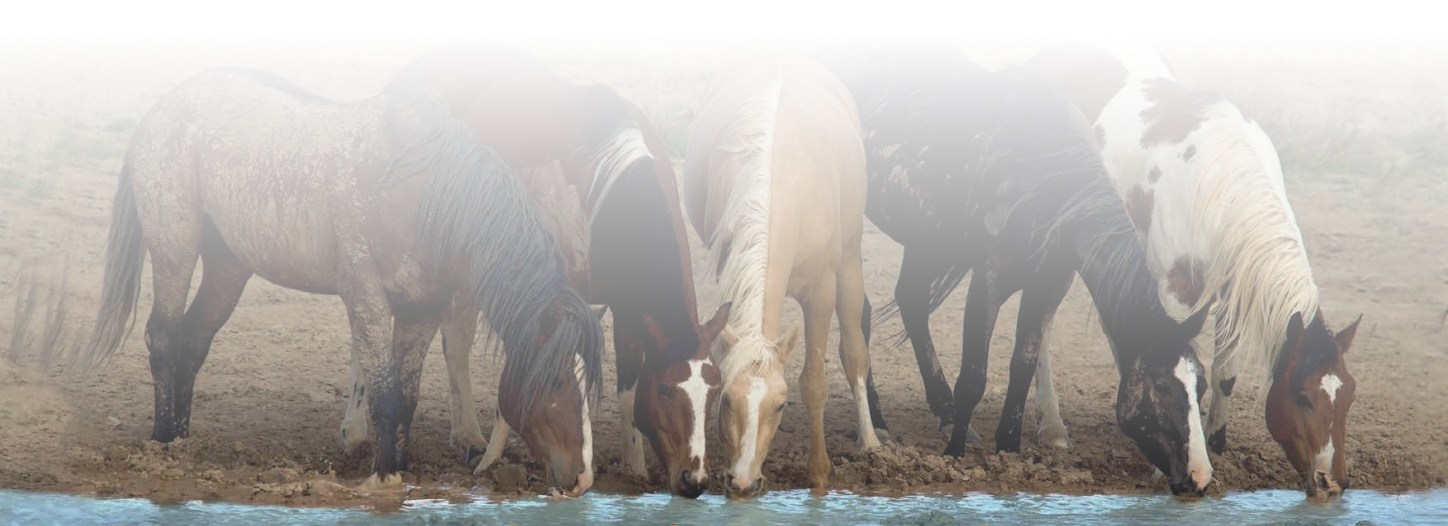
\includegraphics[width=\paperwidth]{topos-horses}\end{minipage}}
\begin{frame}[c]
  \centering

  \bigskip
  %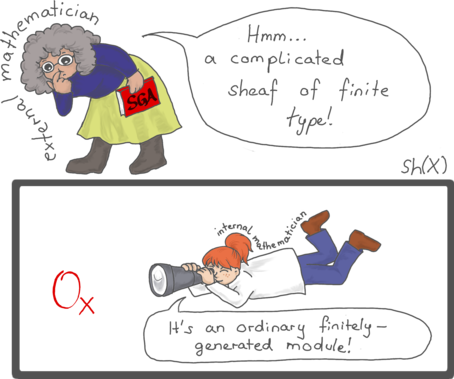
\includegraphics[width=0.4\textwidth]{external-internal-small}
  \bigskip
  \bigskip
  \bigskip
  \bigskip
  \bigskip
  \bigskip
  \bigskip
  \bigskip

  \hil{Without loss of generality, \\ any reduced ring is a field}

  \scriptsize
  \textit{-- an invitation --}
  \bigskip
  \bigskip
  \bigskip
  \bigskip
  \bigskip
  \bigskip
  \bigskip

  \color{blue!80}REDCOM: \\ \emph{Reducing complexity in algebra, logic, combinatorics} \\
  \color{black}
  \medskip
  online via Università degli Studi di Verona \\
  February 2nd, 2022

  \bigskip
  \bigskip

  \color{black}
  Ingo Blechschmidt \\
  University of Augsburg
  \bigskip
  \bigskip
  \bigskip

  \par
\end{frame}}

\begin{frame}{Transfinite methods in algebra?}
  Let~$A$ be a ring which is reduced: If~$x^n = 0$, then~$x = 0$.

  \subhead{Injective matrices}
  \begin{varblock}{\textwidth}{Injective matrices}
    \justifying
    \textbf{Theorem.}
    Let~$M$ be an injective matrix with more columns than rows over~$A$.
    Then~$1 = 0$ in~$A$.
  \end{varblock}

  \justifying
  \visible<2->{\textbf{Proof.} \bad{Assume not.}} \visible<3->{Then there is a \bad{minimal
  prime ideal} $\ppp \subseteq A$.} \visible<4->{The matrix is injective over
  the \bad{field}~$A_\ppp$;} \visible<5->{contradiction to basic linear algebra. \qed}\medskip
  \bigskip

  \only<1-5>{\centering\bigskip\bigskip\scalebox{0.8}{$\begin{pmatrix}
    \cdot & \cdot & \cdot & \cdot & \cdot \\
    \cdot & \cdot & \cdot & \cdot & \cdot \\
    \cdot & \cdot & \cdot & \cdot & \cdot
  \end{pmatrix}$}\par}

  \only<4-5>{
    \begin{align*}
      A_\ppp &= A[S^{-1}] = \{ \tfrac{x}{s} \,|\, x \in A, s \not\in \ppp \} && \text{where $S = A \setminus \ppp$} \\
      A[f^{-1}] &= A[S^{-1}] = \{ \tfrac{x}{f^n} \,|\, x \in A, n \geq 0 \} && \text{where $S = \{f^0,f^1,\ldots\}$}
    \end{align*}
  }

  \pause
  \pause
  \pause
  \pause
  \pause

  \subhead{Grothendieck's generic freeness}
  \begin{varblock}{\textwidth}{Generic freeness\phantom{p}}
    \justifying
    \textbf{Theorem.}
    Let~$M$ be a finitely generated~$A$-module.
    If~$f = 0$ is the only element of~$A$ such that~$M[f^{-1}]$ is a
    free~$A[f^{-1}]$-module, then~$1 = 0$ in~$A$.
  \end{varblock}

  \justifying
  \textbf{Proof.} See \href{https://stacks.math.columbia.edu/tag/051Q}{[Stacks Project]}. \qed

  \centering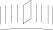
\includegraphics[width=0.25\textwidth]{generic-freeness}
\end{frame}

{\usebackgroundtemplate{\begin{minipage}{\paperwidth}\vspace*{5.95cm}
\includegraphics[width=\paperwidth]{fr1}\end{minipage}}
\begin{frame}{A remarkable sheaf}
  \justifying
  Let~$A$ be a ring.
  Then there is a certain related \speak{ring}~$A^\sim$ such that \ldots
  \bigskip

  \subhead{$\boldsymbol{A^\sim}$ is close to~$\boldsymbol{A}$}
  \begin{enumerate}
  \item
    $A^\sim$ inherits any property of~$A$ which is
    \hil{localization-stable}.
  \item
    A geometric sequent holds for~$A^\sim$ iff$^\star$ it holds for \hil{all
    stalks}~$A_{\mathfrak{p}}$.
  \end{enumerate}
  \bigskip

  \subhead{$\boldsymbol{A^\sim}$ is better than~$\boldsymbol{A}$}
  {\small\centering(Now assume~$A$ reduced.)\par}
  \begin{enumerate}[a]
  \item $A^\sim$ is a \hil{field}: $\forall x\?A^\sim\_ (\neg(\exists y\?A^\sim\_
    xy = 1) \Rightarrow x = 0)$.

  \item $A^\sim$ has \hil{$\boldsymbol{\neg\neg}$-stable equality}:
    $\forall x,y\?A^\sim\_ \neg\neg(x = y) \Rightarrow x = y$.

  \item \mbox{$A^\sim$ is \hil{anonymously Noetherian}.}\\[-1.2em]
  \end{enumerate}

  \begin{varblock}{0.7\textwidth}{}
  {\centering This sheaf can be exploited to give short, \\ conceptual and
  constructive proofs.\par}
  \end{varblock}
\end{frame}}


\newcommand{\eff}{\only<2->{f}}
\newcommand{\ondf}{\only<2->{ on~$D(f)$}}
\newcommand{\fone}{\only<1>{1}\only<2->{f}}
\newcommand{\fonen}{\only<1>{1}\only<2->{f^n}}
\begin{frame}{The sheaf model as a local lens}
  \vspace*{-1.2em}
  \small
  \renewcommand{\arraystretch}{1.3}
  \begin{tabular}{p{0.31\textwidth}p{0.75\textwidth}}
    \hil{sheaf model~$\boldsymbol{A^\sim}$} & \hil{ring~$\boldsymbol{A}$} \\
    \speak{$(\forall x\?A^\sim\_ \varphi(x))$\ondf} &
      for all~$g \in A$ and~$x \in A[g^{-1}]$, \speak{$\varphi(x)$ on~$D(\eff g)$} \\
    \speak{$\varphi \Rightarrow \psi$\ondf} &
      for all~$g \in A$, \speak{$\varphi$ on~$D(\eff g)$} implies~\speak{$\psi$ on~$D(\eff g)$} \\
    \speak{$\varphi \vee \psi$\ondf} &
      there is a partition~$\fonen = \eff g_1{+}\cdots{+}\eff g_m$ s. th.
      for each~$i$, \phantom{lolololl} \phantom{lololo}\speak{$\varphi$ on~$D(\eff g_i)$} or \speak{$\psi$ on~$D(\eff g_i)$} \\
    \speak{$\bot$\ondf} & \only<1>{$1 = 0$ in~$A$}\only<2->{$\fone$ is nilpotent}
  \end{tabular}
  \bigskip
  \pause
  \pause


  \subhead{On the field property}

  Let~$x \in A$ be such that
  \[ \text{\speak{$x \in A^\sim$ is not invertible on~$D(1)$}}, \]
  that is \pause
  \[ \text{\speak{$(\text{$x \in A^\sim$ is invertible}) \Rightarrow \bot$ on~$D(1)$}}, \]
  that is \pause
  \[ \text{for all~$g \in A$, if \speak{$x \in A^\sim$ is invertible on~$D(g)$}
  then~\speak{$\bot$ on~$D(g)$}}, \]
  that is \pause
  \[ \text{for all~$g \in A$, if $x$ is invertible in~$A[g^{-1}]$
  then~$g$ is nilpotent}. \] \pause
  Then, considering~$g \defeq x$, it follows that~$x = 0$ in~$A$.

%  \begin{align*}
%    & \text{\speak{$x$ is not invertible on~$D(1)$}, that is} \\
%    & \text{\speak{$(\text{$x$ is invertible}) \Rightarrow \bot$ on~$D(1)$}, that is} \\
%    & \text{for all~$g \in A$, if \speak{$x$ is invertible on~$D(g)$} then~\speak{$\bot$ on~$D(g)$}, that is} \\
%    & \text{for all~$g \in A$, if $x$ is invertible in~$A[g^{-1}]$
%  then~$g$ is nilpotent;}
\end{frame}

\begin{frame}{Revisiting the test cases}
  \subhead{Injective matrices}
  \begin{varblock}{\textwidth}{Injective matrices}
    \justifying
    \textbf{Theorem.}
    Let~$M$ be an injective matrix with more columns than rows over a ring~$A$.
    Then~$1 = 0$ in~$A$.
  \end{varblock}

  \justifying
  \textbf{Proof.} \bad{Assume not.} Then there is a \bad{minimal
  prime ideal} $\ppp \subseteq A$. The matrix is injective over the \bad{field}~$A_\ppp$;
  contradiction to basic linear algebra.\qed\medskip

  \textbf{Proof.} \speak{$M$ is also injective as a matrix over~$A^\sim$.
  This is a contradiction by basic intuitionistic linear
  algebra.} Thus~\speak{$\bot$}. Hence~$1 = 0$ in~$A$.\qed
  \bigskip
  \pause

  \subhead{Grothendieck's generic freeness}
  \begin{varblock}{\textwidth}{Generic freeness\phantom{p}}
    \justifying
    \textbf{Theorem.}
    Let~$M$ be a finitely generated~$A$-module.
    If~$f = 0$ is the only element of~$A$ such that~$M[f^{-1}]$ is a
    free~$A[f^{-1}]$-module, then~$1 = 0$ in~$A$.
  \end{varblock}

  \justifying
  \textbf{Proof.} The claim amounts to \speak{$M^\sim$ is \hil{not not} free}.
  This statement follows from basic intuitionistic linear algebra over the
  field~$A^\sim$.\qed
\end{frame}


\backupstart

\begin{frame}{Forcing locality}
  \begin{varblock}{\textwidth}{}
    \justifying
    \textbf{Definition.} A ring is \hil{local} iff~$1 \neq 0$ and~$x + y = 1$
    implies that~$x$ is invertible or~$y$ is invertible.
  \end{varblock}

  \textbf{Examples:}\phantom{Non-}\,\! $k,\ k[[X]],\ \CC\{z\},\ \ZZ_{(p)}$ \\[0.2em]
  \textbf{Non-examples:} $\ZZ,\ k[X],\ \ZZ/(pq)$

  Not every ring~$A$ is local. But always: \speak{$A^\sim$ is local on~$D(1)$}

  Locally, any ring is local: Let~$x + y = 1$ in a ring~$A$.
  Then:
  \begin{itemize}
    \item The element $x$ is invertible in~$A[x^{-1}]$.
    \item The element $y$ is invertible in~$A[y^{-1}]$.
    \item $(D(x), D(y))$ \emph{covers}~$D(1)$.
  \end{itemize}
\end{frame}

\backupend

\end{document}
